\section{Proof Of Concept}



\subsection{Anforderungen}

\begin{itemize}
    \item  Als <Sender Rolle> möchte ich Notifikationen versenden können. 
    \item Als <Empfänger Rolle> möchte ich Notifikationen in der Applikation sehen, wenn die Applikation geöffnet ist.  
    \item Als <Empfänger Rolle> möchte ich Notifikationen über das OS erhalten, wenn die Applikation minimiert ist. 
\end{itemize}

\subsection{Restriktionen}

\begin{itemize}
    \item Nur 1 Client. 
    \item Nur 1 fixe Notifikation. Keine Types. 
    \item Notifikation wird vom Client gesendet und vom selben Client empfangen. 
    \item Keine Authentication oder Authorization. 
  
\end{itemize}



\subsection{Architektur}


\subsection{Messaging Service}



\subsubsection{Überblick}

Für den Proof Of Concept wird eine vereinfachte Architektur aufgebaut. Für den Proof Of Concept sehen wir drei Applikationen vor: 

\begin{itemize}
    \item Messaging Service
    \item Cloud Service
    \item Mobile Client
\end{itemize}


\begin{figure}[H]
\centering
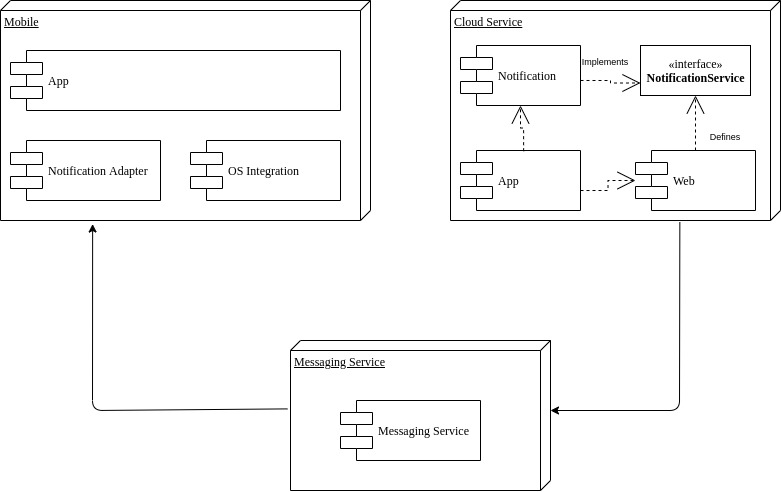
\includegraphics[width=\linewidth]{IP5_POC_Cloud_Architecture.jpg}
\end{figure}




\subsection{Messaging Service}

Dies wird ein externer Service den wir in die Applikationen einbinden. Standard hierfür ist Firebase Notifications. 

Der Messaging Service nimmt Notifikationen vom Cloud Service entgegen und gibt diese an den Mobile Client wieder. 

Dafür müssen auf beiden Seiten Komponenten eingebaut werden, die mit dem Messaging Service kommunizieren. 



\subsection{Cloud Service}

Der Cloud Service für den POC ist in drei Module unterteilt: 

App - Dieses Modul fasst die anderen Module zusammen und bietet die Funktionalität den Service zu starten. Im Build Prozess es dieses Modul, dass am Ende das deploybare Artifakt liefert. 

Web - Dieses Modul bietet eine REST SChnittstelle nach aussen die von einem Client angesprochen werden kann. Diese Schnittstelle bietet die Möglichkeit eine Notification zu senden. Dazu definiert das Web Modul ein Interface "NotificationService"

Notification - Dieses Modul implementiert das NotificationService Interface aus dem Web Modul. In der Implementation wird die Integration an den Message Service implementiert. 




\subsection{Mobile Client}

Der Mobile Client implementiert die Anbindung an den Messaging Service. 

Als Reaktion auf eine Notification wird eine OS Push Notifikation gesendet. 

Als Reaktion auf eine Notification wird eine Rückmeldung im UI angezeigt. 

Das UI bietet einen Button der eine Anfrage an die REST Schnittstelle im Cloud Service sendet. 



\clearpage
